\chapter{内存寻址}

\section{内存地址}

    在使用80x86微处理器时,我们必须区分以下三种不同的地址:

\begin{itemize}
    \item 逻辑地址(logical address)
    \subitem 包含在机器语言指令中用来指定一个操作数或一条指令的地址。\emph{每一个逻辑地址都由一个段(segment)和偏移量(offset或displacement)组成,偏移量指明了从段开始的地方到实际地址之间的距离。}
    \item 线性地址(linear address)(也称虚拟地址 virtual address)
    \subitem 是一个32位无符号整数,可以用来表示高达4GB的地址。
    \item 物理地址(physical address)
    \subitem 用于内存芯片级内存单元寻址。从微处理器的地址引脚发送到内存总线上的电信号相对应。
\end{itemize}

    \emph{内存控制单元(MMU)通过分段单元(segmentation unit)的硬件电路把一个逻辑地址转换成线性地址,然后分页单元(paging unit)的硬件电路把线性地址转化为物理地址}。

    在多处理器中,所有CPU都共享同一内存:这意味着RAM可以由独立的CPU并发访问。但因为RAM上的读写必须串行执行,因此需要内存仲裁器(memory arbiter)的硬件电路插在总线和RAM芯片之间。

    内存仲裁器的作用是:\emph{如果某个RAM空闲,就准予CPU访问。若RAM忙于另一个CPU提出的请求服务,就延迟这个CPU的访问}

\section{硬件中的分段}

    从80286模型开始,Intel处理器以实模式\footnote[1]{\emph{实模式(Real Mode)是x86体系结构中的一种工作模式,它是早期x86处理器的默认工作模式。在实模式下,处理器以16位的方式进行操作,可以直接访问1MB的物理内存。在实模式下,内存寻址是通过段地址和偏移地址的组合来实现的。段地址由段寄存器(如CS、DS、ES等)保存,偏移地址由指令中的操作数给出。通过将段地址左移4位后与偏移地址相加,可以计算出实际的物理地址}}(real mode)和保护模式(protected mode)执行地址转换。

\subsection{段选择符和段寄存器}

    一个逻辑地址由\emph{一个段标识符(16位长的字段,段选择符(Segment Selector))和一个指定段内相对地址的偏移量(32位长的字段)组成。}

\begin{figure}[!htbp]
    \centering
    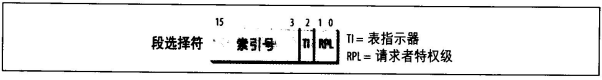
\includegraphics[width=0.8\textwidth]{image/chapter02/段选择符格式.png}
    \caption{段选择符格式}
\end{figure}

    为了方便段选择符,段寄存器用于存放段选择符。其拥有六个寄存器:

\begin{table*}[!htbp]
    \begin{center}
        \begin{tabular}{c | c}
            cs & 代码段寄存器,指向包含程序指令的段 \\
            ss & 栈段寄存器,指向包含当前程序栈的段 \\
            ds & 数据段寄存器,指向包含静态数据或者全局数据段 \\
            es, fs, gs & 一般用途,可以指向任意数据段 
        \end{tabular}
    \end{center}
\end{table*}

    cs寄存器:\emph{包含一个两位的字段,用以指明CPU的当前特权级\footnote[1]{\emph{值为0表示最高优先级,值为3为最低。Linux只用0和3表示内核态和用户态。}}(Current Privilege Level, CPL)。}

\subsection{段描述符}

    每个段由一个8字节的段描述符(Segment Descriptor)表示,描述了段的特征。

    段描述符放在全局描述符表(Global Descriptor Table,GDT)或局部描述符表(Local Descriptor Table,LDT)中。

    通常只定义一个GDT,每个进程除了存放在GDT中的段之外如果还需附加,就可以使用LDT。GDT在主存中的地址和大小存放在gdtr控制寄存器中,LDT地址和大小存放在ldtr控制寄存器中。

\begin{table*}[!htbp]
    \begin{center}
        \caption{段描述符字段}
        \begin{tabular}{c l}
            \hline
            \emph{字段名} & \emph{描述} \\
            Base & 包含段的首字节的线性地址 \\ 
            G & 粒度标志;若清零,则段大小以字节为单位,否则以4096字节倍数计 \\
            Limit & 存放段中最后一个内存单元的偏移量,从而决定段的长度。\\
            S & 系统标志;置零表示系统段,否则是普通代码段或数据段 \\
            Type & 描述了段的类型特征和存取权限 \\
            DPL & 描述符特权级(Dsecriptor Privilege Level)字段;用于限制这个段的存取。\\
            & 其表示为访问这个段要求的CPU最小优先级。若DPL设为0的段只能\\
            & 当CPL为0时(即内核态)可访问 \\
            P & Segment-Present标志;等于0表示段当前不在主存中\\ 
            & \emph{Linux总是把这个标志设置为1,因为其从不把整个段交换到磁盘}\\
            D或B & 取决于是代码段还是数据段。D或B的含义在两种情况下略有区别\\
            & 如果偏移量32位则置1,否则清零 \\
            \hline
        \end{tabular}
    \end{center}
\end{table*}

    有几种不同类型的段以及对应的段描述符:

\begin{itemize}
    \item 代码段描述符
    \subitem 表示这个段描述符表示代码段,S标志置1
    \item 数据段描述符
    \subitem 表示这个段描述符表示数据段,S标志置1
    \item 任务状态段描述符(TSSD)
    \subitem 表示这个段描述符表示任务状态段(Task State Segment, TSS),也就是该段用于保存处理器寄存器的内容。\emph{只能出现在GDT中,根据相应进程是否在CPU上,其Type字段值为11或9,S标志置零}
    \item 局部描述符表描述符(LDTD)
    \subitem 表示这个段描述符包含一个LDT段,其只出现在GDT中。相应的Type字段值为2,S标志置0
\end{itemize}

\begin{figure}[!htbp]
    \centering
    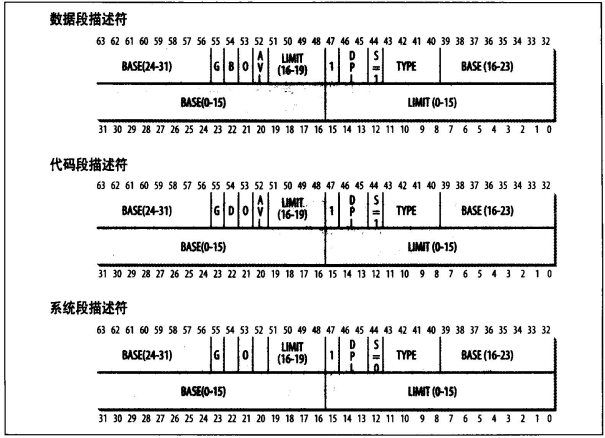
\includegraphics[width=0.8\textwidth]{image/chapter02/段描述符格式.png}
    \caption{段描述符格式}
\end{figure}

\subsection{快速访问段描述符}

    \emph{逻辑地址由16位段选择符和32位偏移量组成,段寄存器仅仅存放段选择符。}

    为了加速逻辑地址$\rightarrow$线性地址,80x86处理器提供了附加的非编程的寄存器,供6个可编程的段寄存器使用。每一个非编程的寄存器含有八个字节的段描述符,由对应的段寄存器中的段选择描述符来指定。

    每当一个段选择符被装入段寄存器,相应的段描述符就由内存装入对应的非编程CPU寄存器。这时,针对该段的逻辑地址转换就可以仅访问该非编程寄存器即可(除非段寄存器内容发生更改)。

\begin{figure}[!htbp]
    \centering
    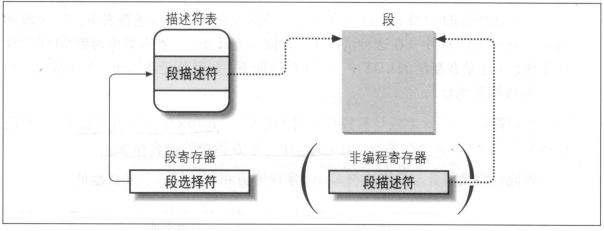
\includegraphics[width=0.8\textwidth]{image/chapter02/段选择符和段描述符.png}
    \caption{段选择符和段描述符}
\end{figure}

\begin{table*}[!htbp]
    \begin{center}
        \caption{段选择符字段}
        \begin{tabular}{c l}
            \hline
            \emph{字段名} & \emph{描述} \\
            index & 指定了描述放在GDT/LDT中对应的段描述符入口 \\
            TI & TI((Table Indicator)标志,指明段描述符是在GDT(TI = 0)中或LDT(TI = 1)中) \\
            RPL & 请求者特权级,当相应的段选择符装入到cs寄存器中时指示出CPU当前的特权级 \\
            & 还可以用于访问数据段时选择地削弱特权级 \\
            \hline
        \end{tabular}
    \end{center}
\end{table*}

    由于段描述符是8字节长,因此在GDT/LDT中的相对地址由段选择符的最高13位数值乘以8得到

    \emph{GDT的第一项总是设置为0,这就确保了空段选择符的逻辑地址会被认为是无效的。因此引起一个处理器异常。}

\subsection{分段单元}

    分段单元(segmentation unit)执行以下步骤:

\begin{itemize}
    \item 首先检查TI字段以决定段描述符保存在哪个描述符表。
    \item 从段选择符的index字段计算段描述符的地址
    \item 把逻辑地址的偏移量与段描述符Base字段的值相加就得到了线性地址
\end{itemize}

\begin{figure}[!htbp]
    \centering
    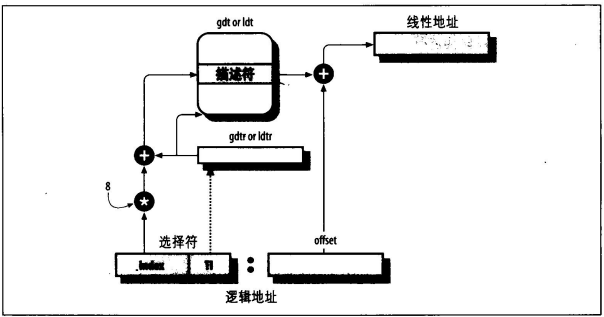
\includegraphics[width=0.8\textwidth]{image/chapter02/逻辑地址的转换.png}
    \caption{逻辑地址的转换}
\end{figure}

    注意:\emph{如果有了不可编程寄存器,只有当段寄存器内容被改变时才需执行前两个操作。}